\chapter{Laboratorio 6: \\Functional Verification}
\section{VHDL Testing}
\subsection{A given RCA}
Nella prima parte dell'esperienza di laboratorio viene fornito il \textit{Testbench} di un \textit{Ripple Carry Adder}, contenente un errore.\\
Il Test Bench era diviso sostanzialmente in tre parti:
\begin{itemize}
	\item{Random Input Values}
	\item{Reference Architecture}
	\item{Assert Instructions}
\end{itemize}
All'interno del codice si può notare come una volta generat
\subsection{A more complex case}
Nella seconda parte di questo primo esercizio viene richiesto di verificare la correttezza di quattro versioni di un circuito \textit{incrementer$\&$comparator} presente in Figura \ref{pentium}.
\begin{figure}[!htb]
	\centering
	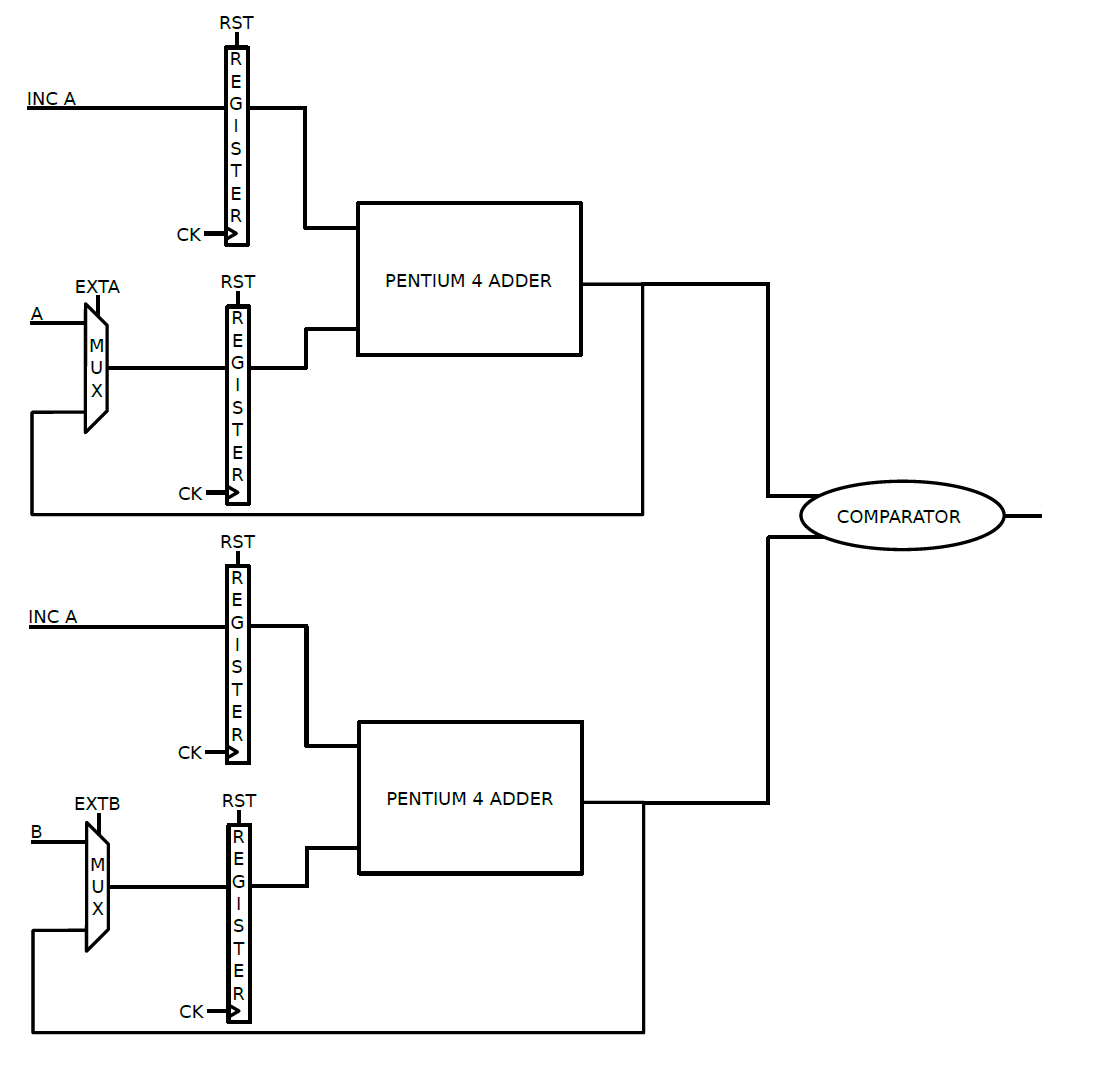
\includegraphics[scale=1]{immagini/pentium}
	\caption{\textit{Probabilità e Switching Activity stimati manualmente}}
	\label{pentium}
\end{figure}
La struttura presenta 4 blocchi diversi, replicati due volte, e un compatore:
\begin{itemize}
	\item  Due multiplexer a due vie che selezionano l'ingresso \textit{A} e \textit{B} oppure l'uscita del rispettivo sommatore con poi un Registro in uscita
	\item un registro per campionare l'ingresso \textit{INCA} e \textit{INCB} che decide se incrementare o meno l'ingresso A e B.
	\item due sommatori, realizzati tramite la struttura \textit{Pentium 4 Adder}
	\item un comparatore che manda in uscita il valore maggiore tra A e B
\end{itemize}
Dopo aver letto il funzionamento del Pentium 4 tramite l'appendice si è iniziata la realizzazione del TestBench per scoprire quali fossero i bug presenti. Veniva fornita una versione di riferimento del circuito, priva di bug in modo da avere un'architettura di riferimento con la quale confrontare le 4 versioni del circuito.\\
Il VHDL implementato per questo scopo è presente in Figura \ref{testbench_vhdl1} e \ref{testbench_vhdl2}.
\begin{figure}[!htb]
	\centering
	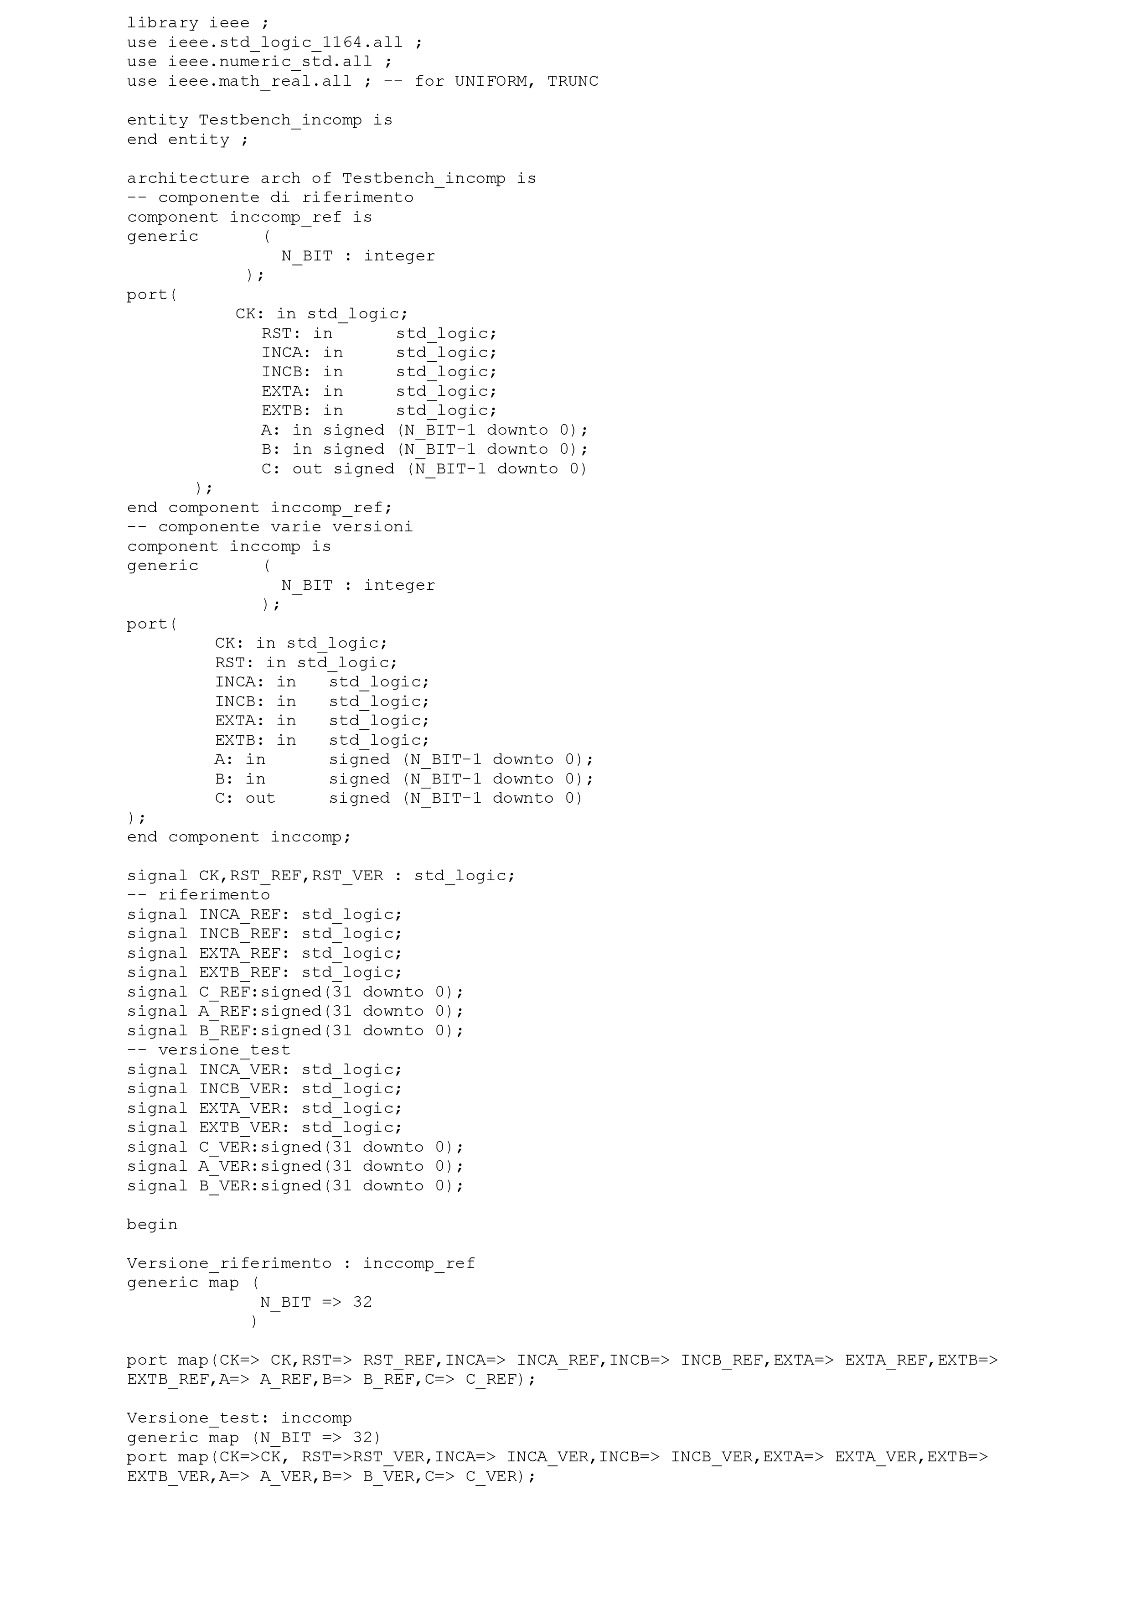
\includegraphics[scale=0.3]{immagini/testbench_vhdl1}
	\caption{\textit{Probabilità e Switching Activity stimati manualmente}}
	\label{testbench_vhdl1}
\end{figure}
\begin{figure}[!htb]
	\centering
	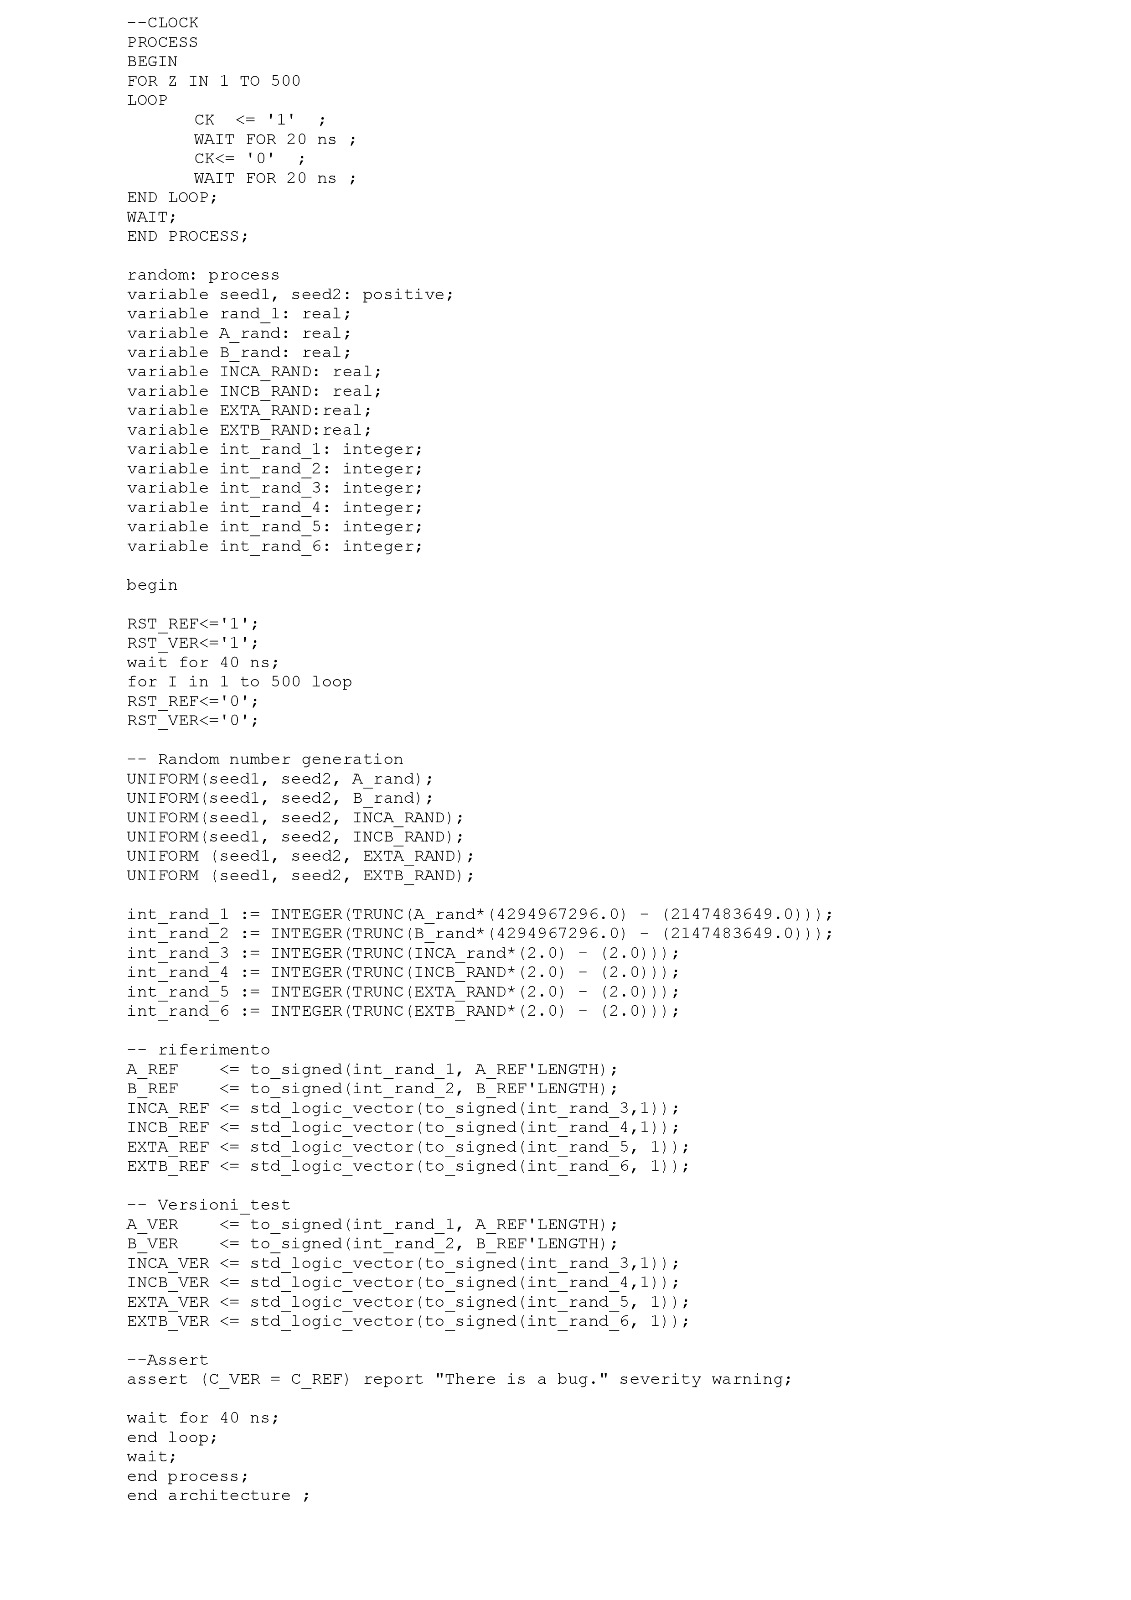
\includegraphics[scale=0.3]{immagini/testbench_vhdl2}
	\caption{\textit{Probabilità e Switching Activity stimati manualmente}}
	\label{testbench_vhdl2}
\end{figure}
\newpage
\noindent La struttura del Testbench è simile a quella fornita nell'esercizio precedente.\\
Ho una prima parte di generazione di numeri casuali, nello specifico genero in modo assolutamente randomico gli ingressi A e B, i selettori dei multiplexer EXTA e EXTB e gli ingressi di incremento INCA e INCB.\\
In realtà simulando attentamente il circuito ci si è resi conto di come la soluzione con numeri random non sia sempre ottimale per la ricerca di un bug, in quanto, specialmente nel caso di un ingresso con un numero di bit molto elevato, sono necessarie numerose iterazioni per provare tutte le possibili combinazioni. Questo sta alla base della mancato ritrovo del bug nella quarta versione, in quanto tramite un Testbench con numeri random non siamo riusciti a "sollecitare" l'errore: probabilmente si sarebbe dovuto studiare degli ingressi opportuni per sollecitare il sommatore in modo più specifico.\\
La seconda parte del TestBench prende gli ingressi sviluppati nella parte prima e genera le uscite sia dell'architettura di riferimento che della versione da analizzare.\\
Infine viene effettuato il confronto tra le due uscite e viene definita una funzione di \textit{assert} che fornisce sul \textit{Transcript} di Modelsim un messaggio di errore nel caso in cui venga rilevato un bug.
Nella prima versione del circuito risulta un errore all'interno di un multiplexer presente nel selettore di riporto del sommatore, in quanto l'ingresso riferito all' '1' e allo '0' risultavano invertiti. Questa prima versione ha un errore molto "visibile" e facile da trovare, sono state necessarie quindi pochissime iterazioni.\\
Nella seconda versione del circuito invece, risulta un errore nel selettore del multiplexer del sommatore, in quanto invece di assegnare
\begin{center}
	$C\_IN(N\_BIT/CARRY-1)$
\end{center} 
assegna 
\begin{center}
	$C\_IN(N\_BIT/CARRY-2)$
\end{center}
Per trovare quest'errore sono state necessarie 500000000 iterazioni, un numero già ritenuto eccessivo. Si riporta in allegato in Figura \ref{sim1} la simulazione Modelsim contenente l'errore.
\begin{figure}[!htb]
	\centering
	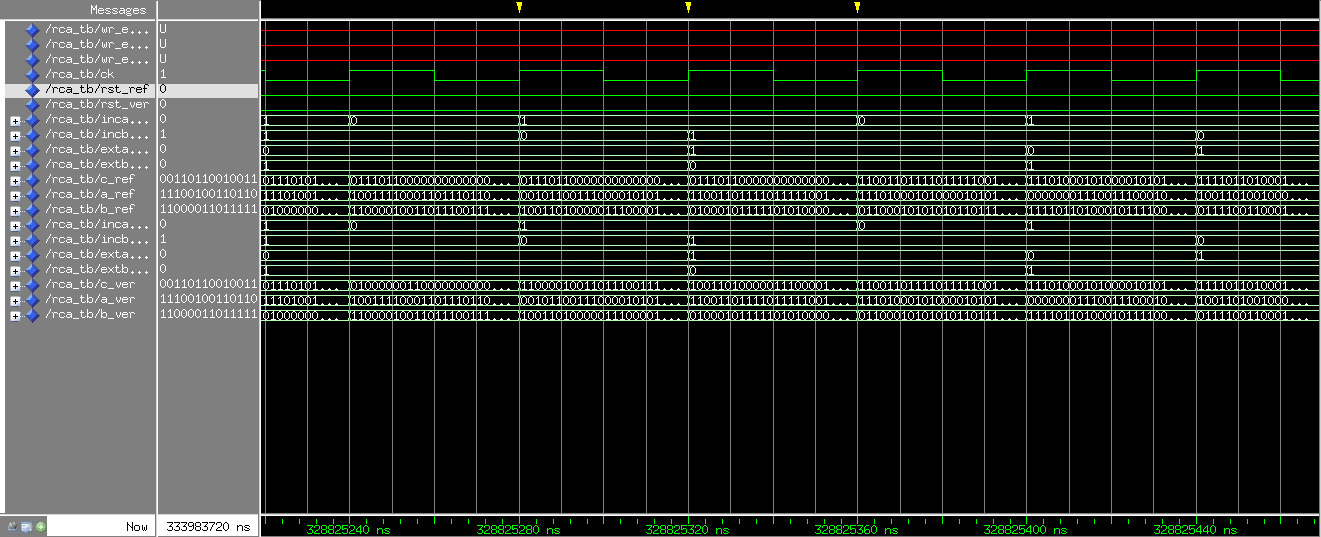
\includegraphics[scale=0.6]{immagini/sim1}
	\caption{\textit{Probabilità e Switching Activity stimati manualmente}}
	\label{sim1}
\end{figure}
\\
\\
\\
\\
\\
\\
\\
\\
\\
\\
\subsection{Finite State Machine}
Questa parte prevede di testare il  funzionamento di una FSM (Macchina a stati finiti), disponibile in 4 versioni differenti, contenenti dei bug.  
La FSM da testare è, un contatore up/down a 3 bit, la FSM è la seguente:
\begin{figure}[!htb]
	\centering
	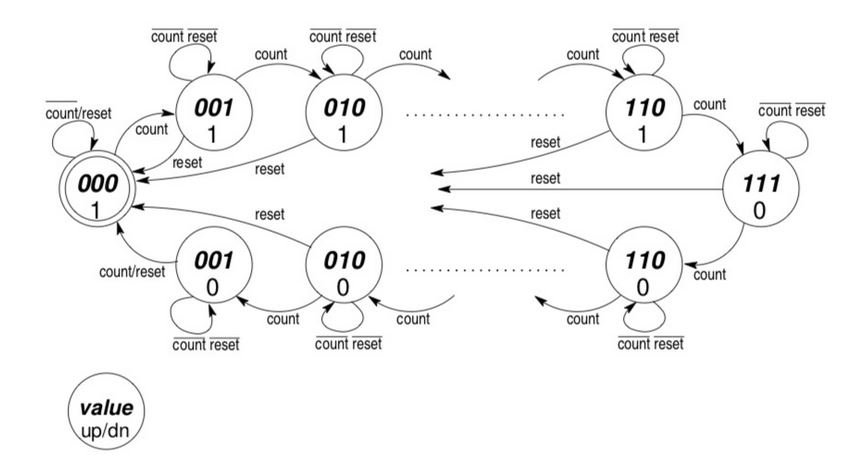
\includegraphics[scale=0.8]{immagini/fsm_lab6}
	\caption{\textit{Macchina a stati da testare}}
	\label{Fsm, up-down counter}
\end{figure}
\\
\\
\\
\\
Prendendo spunto dal punto precedente il test è stato realizzato mediante i seguenti file:\\
\textit{counter\_ref.vhd}, è il file del contatore dal corretto funzionamento, utilizzato per calcolare le uscite corrette da confrontare successivamente.
\\
\textit{counter.vhd}, è il dispositivo da testare, disponibile in 4 versioni, site in diverse cartelle, poi estratte da modelsim volta per volta durante la simulazione
\\
\textit{counter\_tb.do}, è lo script che si occupa di dirigere la compilazione e simulazione dei 4 files da testare su Modelsim, in cui è impostata anche la durata della simulazione e la visualizzazione delle forme d’onda dei segnali rilevanti ai fini della verifica, per consentire una comoda visione dell’andamento temporale dei segnali.
Di seguito un estratto del file disponibile in appendice.\\
\\
.......\\
.......\\
echo "testing v1..."\\
\\
vcom -reportprogress 300 -work work\\ /home/lp19.12/repository/lab6/ese6/3/counter\_tb.vhd\\ /home/lp19.12/repository/lab6/ese6/3/vREF/counter\_ref.vhd\\ /home/lp19.12/repository/lab6/ese6/3/v1/counter.vhd\\
\\
vsim -t ns -novopt work.counter\_tb\\
\\
set NumericStdNoWarnings 1\\
run 0 ps\\
set NumericStdNoWarnings 0\\
\\
add wave -radix binary   -color BLUE\\      sim:/counter\_tb/DATA\_OUT\_tb\\
add wave -radix binary   -color GREEN\\    sim:/counter\_tb/DATA\_OUT\_ref\\
add wave -radix binary   -color BLUE\\     sim:/counter\_tb/UP\_DN\_tb\\
add wave -radix binary   -color GREEN \\   sim:/counter\_tb/UP\_DN\_ref\\
run 30000000 ns\\
\\
echo "end v1"\\
.......\\
.......\\
\\
\\
\\
\textit{counter\_tb.vhd}, ile di testbench che si occupa di:
\begin{itemize}
	\item {generare gli ingressi e definire i componenti: il REF, dispositivo di riferimento utilizzato per calcolare le uscite corrette a partire dagli ingressi generati; il DUT (device under test), il contatore da verificare che sarà rappresentato di volta in volta nella simulazione da uno dei quattro circuiti da testare.}
	\item {generare il segnale di clock e i gli ingressi generati in modo pseudo-casuale.}
	\item {confrontare le uscite dei due dispositivi per rilevare possibili errori e segnalarli con un apposito messaggio.}
\end{itemize}
Di seguito sono riportate le parti più significative del file di testbench, disponibile integralmente in appendice.\\
\\
.......\\
.......\\
for I in 1 to 50000 loop\\
-- Random number generation\\
UNIFORM(seed1, seed2, rand);\\
\\
std\_rand:=std\_logic\_vector(to\_unsigned(integer(rand), 2));\\
\\
COUNT\_TB    <= std\_rand(0);\\
RST\_TB    <= std\_rand(1); \\
\\
-- Assert\\
wait for 2 ns;\\
assert (DATA\_OUT\_TB=DATA\_OUT\_REF) report "There is a bug in result." severity warning;\\
assert (UP\_DN\_TB=UP\_DN\_REF) report "There is a bug in UP\_DN signal" severity warning;\\
wait for 10 ns;\\
end loop;\\
wait;\\
………\\
………\\
\\
E' evidente come testare una macchina a stati sia più complicato e dispendioso dal punto di vista del testing rispetto all'analisi di un circuito combinatorio, visto che si devono tenere in considerazione anche gli stati precedenti.\\ 
\section{Scripting in Python}
\subsection{Automatic verification through a script}
Un modo per automatizzare il processo di verificare è realizzare uno script python che consente una verifica più veloce ed efficace. Lo scopo della prima parte è quella di completare il template del file testing\_script.py, per testare il circuito del RCA utilizzato nella prima parte del laboratorio.\\
il file testing\_script.py  si compone di 5 parti:
\begin{itemize}
	\item{generazione degli input file in formato .txt da mandare poi al DUT}
	\item{lancio della simulazione Modelsim tramite comandi bash}
	\item{calcolo dei risultati tramite algoritmo di python che servirà a fornire i valori di riferimento per il confronto con i valori  di uscita del dut}
	\item{prelievo dei risultati della simulazione modelsim salvati su file \textit{output\_data.txt}}
	\item{comparazione dei risultati ottenuti da modelsim con quelli di riferimento calcolati da python}
\end{itemize}
Per la generazione pseudo-casuale degli input si è utilizzata la struttura, già fornita nel file \textit{generate\_inputs.py}:\\
\\
………\\
......\\
\# Loop for all steps\\
for i in range(0,NumberOfSteps):\\
\# Loop for all signals\\
for i in range (0, SignalsNumber):\\
\# Generate integer number\\
RandomInputInteger = randint(1,2**GenericsAssignedValue[i]-1)\\
\# Convert number to binary\\
RandomInputBinary = ('{0:0{l}b}'.format((RandomInputInteger),l=GenericsAssignedValue[i]))\\
\# Write file\\
Filepointer.write(RandomInputBinary + " ")\\
\# Write line termination\\
Filepointer.write("\\n")\\
………\\
……\\
\\
La funzione \textit{randint()} permette di generare un intero pseudocasuale entro il range fornito.
Il metodo \textit{format()} permette di convertire l’intero in binario in base al parallelismo degli ingressi definito nella lista \textit{GenericsAssignedValue}.\\
\\
Per quanto riguarda il lancio della simulazione Modelsim, il codice è già stato fornito e si compone di istruzioni bash richiamate tramite il modulo \textit{os} contenente la funzione \textit{system()}.
\\
Lo script si occupa di eliminare eventuali working directories ed input file, impostare le environment variables, e far partire la compilazione e simulazione di Modelsim.
Il testo è disponibile in appendice alla sezione “run modelsim simulation” del file \textit{testing\_script.py}.
\\
Per il calcolo delle uscite con python si è utilizzato il seguente algoritmo:\\
……...\\
……...\\
\#calculate the output values from the inputs generated\\
\#repeat for each set of in's\\
for i in range(0, NumberOfSteps):\\  
\#sum in's\\
Sum=Inputs[i][0]+Inputs[i][1]+Inputs[i][2]\\
\#conversion of the sum in binary\\
SumBin=('{0:b}'.format(Sum))\\
\#conversion in string \\
SumStr=str(SumBin)\\
\#overflow bit preset to '0'\\
Py\_results[i][1]=0 \\
if len(SumStr)!=32:\\
\#management of the overflow\\
if len(SumStr)>32:    \\
SumStr=SumStr[1:]\\
\#overflow bit to '1'\\
Py\_results[i][1]=1\\
else:\\
\#adding zeros to get the value on 32 bit\\
while len(SumStr)<32:  \\
SumStr='0'+SumStr\\
\#re-conversion to successive comparison of the values\\
Py\_results[i][0]=int(SumStr, 2)\\  
………\\
………\\
\\
Al momento della generazione, gli ingressi sono stati salvati nella lista \textit{Inputs[][]}, formata da tutti gli ingressi  generati, raggruppati a gruppi di 3, ogni gruppo corrisponde a uno step di ingressi da calcolare. Si sono sommati gli ingressi e si è poi convertita la somma in binario grazie al metodo \textit{format()}. Per gestire gli overflow e mantenere il parallelismo della somma a 32 bit, si è preferito convertire la somma binaria in stringa in modo da gestire più comodamente il dato nel caso in cui il parallelismo sia variato.
I risultati corretti sono stati salvati nella lista \textit{Py\_results[][]} contenente i gruppi di risultati in intero a coppie di 2 (somma e carry-out), per ogni step di ingressi. I risultati inoltre sono stati salvati nel file \textit{python\_results.txt}\\
\\
Per il prelievo dei risultati della simulazione i dati sono stati prelevati dal file \textit{output\_data.txt} nel quale modelsim ha salvato i valori di uscita. Si è utilizzato lo script già fornito leggendo ogni riga contenente le uscite di ogni step di calcolo tramite un ciclo for.\\ 
……\\
…..\\
\# Open file and acquire data\\
with open(Filename, "r") as f:\\
OutputsBinary = [x.strip().split() for x in f]\\
……..\\
……..\\
\\
Per l’ultima parte, quella che si occupa della comparazione dei risultati, sono stati confrontati in modo ordinato i valori \textit{OutputsDecimal[]} provenienti dalla simulazione con quelli di riferimento salvati in \textit{Py\_results[]} con un ciclo for. Per ogni step, in caso di valori diversi viene stampato un messaggio con l’avviso di errore e lo step i-esimo dell’errore. Inoltre alla fine del confronto viene anche riportato il numero totale di errori riscontrati. Di seguito il codice:\\
\\
……..\\
……..\\
tot\_err=0\\
\#for each results’step\\
for i in range(0, NumberOfSteps):\\
\#comparison the outputs\\
if str(InputsDecimal[i])!=str(Py\_results[i]):\\
\#error message for step “i”    \\
print("found an error in step "+str(i)+"\\n")\\
print(str(InputsDecimal[i]), str(Py\_results[i]))\\
\\
tot\_err=tot\_err+1\\
\#message for total number of errors\\
print("The number of wrong steps is: "+str(tot\_err))\\
………….\\
…………\\
\\
\\
\subsection{Further Generalization}
L’ultima parte prevede di creare uno script che sia in grado di generare un file di testbench a partire dal file .vhd del device under test. Il file contente il codice di generazione del testbench è \textit{tb\_generation.py} file già in parte fornito, che si occupa di:
\begin{itemize}
	\item{leggere il file del dut e salvare tutti i valori utili al testbench, ovvero i generics e gli ingressi e uscite del device. Di seguito un estratto del codice:\\
	…….\\
	…...\\    
	with open(FileName, "r") as fp:\\
	\#save rows\\
	for line in fp:\\
	\#divide the line in words\\
	words=line.strip().split()\\
	\#save words in a list\\
	for w in words:\\
	word.append(w)\\
	\#scanning words to take datas for testbench\\
	while word[i]!="architecture":\\
	if word[i]=="entity":\\
	EntityName=word[i+1]\\
	print EntityName\\
	i=i+3\\
	if word[i]=="generic":\\
	GenericFlag=1\\
	print GenericFlag\\
	i=i+2\\
	while word[i]!=");":\\
	GenericsList.append(word[i])\\
	print GenericsList\\
	i=i+2\\
	GenericsType.append(word[i])\\
	i=i+2\\
	………\\
	……\\}
	\item{creare il file di testbench, eliminando eventuali file con lo stesso nome}
	\item{definire il file di testbench in formato .vhd, utilizzando i dati estratti}
\end{itemize}
Le parti 2 e 3 sono già state fornite, il file completo è comunque disponibile in appendice.
La generalizzazione della creazione del testbench consente di automatizzare ulteriormente il processo di testing del DUT, rendendo lo script più flessibile e adatto a simulazioni future, che grazie a questo file saranno rese più veloci ed efficienti.\\


